\chapter{Аналитический раздел}
\label{cha:analysis}
\section{Цель и задачи работы}
Целью данной работы является создание метода прогнозирования результатов теннисных матчей на основе априорной информации.
Для достижения данной цели необходимо решить следующие задачи:
\begin{itemize}
	
\item проанализировать предметную область и существующие методы прогнозирования результатов теннисных матчей
	\item разработать метод прогнозирования результатов теннисных матчей
	\item создать ПО, обрабатывающее данные для анализа
	\item создать ПО, реализующее  разработанный метод прогнозирования результатов теннисных матчей
\end{itemize}
\section{Сложность прогнозирования результатов}
Спортивное прогнозирование предполагает предугадывание результатов предстоящих спортивных событий или контрольных результатов, которые спортсмен( или команда спортсменов) показывает на спортивных соревнованиях\cite{Book01}. Прогнозы даются на конкретные события в конкретные моменты времени, на результат совокупности событий,ограниченных во времени(например, соревновательный сезон). Наиболее распространены прогнозы на результаты конкретного матча и сезона в целом. Прогнозы могу осуществляться на основе алгоритмов анализа информации, экспертной оценке, а так же комбинацией экспертной оценки. В данной работе будет рассмотрено прогнозирование на основе анализа априорной информации. Это означает, что прогноз на какое-либо событие будет даваться до его начала и текущая информация о ходе события не будет учитываться.


 Большинство исследователей используют различную статистическую информацию для составления прогнозов. Из массива накопленных данных они выбирают небольшое количество наиболее важных показателей(или же останавливаются только на одном из них) за ограниченный промежуток времени, которые подаются на вход алгоритму.
 Какие показатели считать значимыми определяет автор алгоритма на основе экспертной оценки или каких-то дополнительных алгоритмов "отбора наиболее важных показателей\".
 Например, в случае американского футбола\cite{Book02} это могут быть
 \begin{enumerate}
 	\item Время владения мячом
 	\item Проводился ли матч дома или в гостях
 	\item Общее количество ярдов
 	\item Разница в атакующих ярдах
 	\item Количество потерь мяча
 \end{enumerate}
Или же в случае баскетбола, например, может браться следующий набор показателей:
 \begin{enumerate}
	\item  Количество травмированных игроков
	\item Количество выигранных матчей подряд перед данной игроков
	\item Усталость команды. Показатель считается на основе расстояния, которое пришлось преодолеть команде, чтобы провести последние 7 игр
	\item Средний домашний, гостей и общий процент побед
	\item Рейтинг команды в "рейтинге нападения"\ , "рейтинге защиты"\ и "общем рейтинге"\ (подробнее методики подсчёта рейтингов описываются в \cite{Book03})
\end{enumerate}
Большая часть статей представляет команду как некое единое целое, упуская из виду каждого игрока команды. Учёт информации каждом игроке - нетривиальная задача.
Поэтому для упрощения создания алгоритма прогнозирования с учётом каждого игрока команды был выбран вид спорта - одиночный теннис. В каждой команде по одному игроку, два возможных исхода матча - победа или поражения.
% тут явно можно написать больше про
Для понимания специфики теннисного прогнозирования, рассмотрим основные правила игры в теннис, которые могут повлиять на составление алгоритмов прогнозирования. С полной версии правил можно ознакомится на сайте международной теннисной федерации\cite{Book04}.
 \begin{enumerate}
	\item  Мяч должен приземлиться в пределах теннисного поля, чтобы продолжить игру. Если игрок мяч приземляется за пределами поля, то это приводит к потере им очков.
	\item Игроки не могут дотронуться до сетки или перейти на сторону противника
	\item Игроки не могут носить мяч или ловить его ракеткой
	\item Игроки не могут дважды ударить по мячу
    \item Игрок должен дождаться пока мяч пересечёт сетку, прежде чем ударить по нему
    \item Игрок, который не возвращает мяч на половину поля противника, прежде чем он отскочит дважды, считается проигравшим
    \item Если мяч ударяет или касается игроков, то это карается штрафом
    \item Перед тем как отбить подачу, мяч должен отскочить от поля.
    \item Очки -наименьшая единица измерения. Приращение очков идёт в формате 0-15-30-40-гейм.
    \item Гейм состоит из 4 очков и выигрывается, когда игрок набирает 4 очка с преимуществом не менее двух очков.
    \item Сет состоит 6 геймов и выигрывается игроком, который набирает 6 геймов 
 	 с минимальным отрывом в 2 очка.
 	 \item Дополнительный сет - сет, который разыгрывается при достижении игроками счёта 6-6 по геймам. 
  	\item Максимальное количество сетов в матче может достигать 3 или 5. По достижении 2 или соответственно 3 выигранных сетов матч заканчивается.
  	\item "Ровно"\ происходит когда достигнут счёт по очкам 40-40. Чтобы выиграть гейм, игрок должен выиграть два последовательных очка. Если игрок выигрывает одно очко, то счёт в гейме становится "больше"\, но если он теряет следующее очко, то счёт возвращается к "ровно"\ .
  	\item Когда в гейме достигнут счёт 6-6, то играется тай-брейк. В розыгрыше тай-брейке используются особые правила набора очка. Победителей считается игрок, набравший не менее 7 очков с преимуществом два очка над оппонентом.
\end{enumerate}
\section{Основные подходы прогнозирования теннисных матчей}
Существует три основных подхода к прогнозированию теннисных матчей: методы попарного сравнения, методы вычисления очков и методы машинного обучения.
\subsection{Метод подсчёта очков}
Методы вычисления очков(также их называют иерархическими методами) фокусируются на оценке вероятности выигрыша каждого очка в матче. 
% P. K. Newton and J. B. Keller
В этом подходе предполагается, что достаточно знать вероятность выигрыша игроком А $p_a^r$ очка на своей подаче и вероятность выигрыша очка игроком B на своей подаче $p_b^r$. Аналогичные подходы  применяются при подсчете вероятности выигрыша игрока в бадминтоне\cite{Book19} и сквоше\cite{Book20}.Впервые такой метод был применен к теннису в работах Кси и Бюрича\cite{Book21}, Картера и Крю\cite{Book22}, Полларда\cite{Book23}.
Такие работы одинаково определяют вероятность выигрыша очка в матче как равномерную случайную величину, т.е. вероятности  $p_a^r$ и  $p_b^r$ принимаются за постоянные величины на протяжении всего матча. Анализ статистических показателей показывает, что такое предположение допустимо\cite{Book09}, т.к. отклонения от ожидаемой величины невелики.

Игрок А может выиграть гейм у игрока В со счётом [4,0], [4,1],4,2] в случае если игрок А выиграл 4 очка за гейм, а игрок В выиграл не более двух. Если же счёт в гейме стал [3,3], то такая ситуация называется "ровно"\ . В этом случае игрок A может выиграть гейм, закончив его с итоговым счетом [n + 5, n + 3], где $n\geq0$. Чтобы рассчитать вероятность $p_G^R$ выигрыша игроком А гейма на своей подаче, введем следующие обозначения: $p_A^R$ - вероятность выигрыша очка на своей подаче игроком А, $q_A^R=1-p_a^R$, $q_A^G = 1 - p_A^G$, $p_A^G(i,j)$ - вероятность того, что i очков в гейме наберет игрок А, а j очков в гейме наберет игрок B. В результате получим следующую формулу:
\begin{equation}
p_A^G=\sum\limits^{2}_{j=0}{p_A^G(4,j)  + p_A^G(3,3)\sum\limits^{\inf}_{n=0}p_a^{DG}(n + 2, n)}
\end{equation}
Пусть $p_A^{DG}(n + 2, n)$ - вероятность того, что игрок А выиграет с преимуществом в 2 мяча после того как был достигнут счет [3,3] на подаче игрока А.
\begin{equation}
p_A^{DG}(n+2,n)=\sum\limits^{n}_{j=0}{(p_A^Rq_A^R)^j(q^R_Ap^R_A)^{n-j}\frac{n!}{j!(n-j)!}}(p^R_A)^2=(p^R_A)^2(p^R_Aq^R_A)^n2^n
\end{equation}

В результате из формул 1 и 2 можно вывести следующую формулу -  вероятность выигрыша игроком А гейма на своей подаче.
\begin{equation}
p_A^{G} = (p^R_A)^4(1 + 4q^R_A + 10(q^R_A)^2) + 20(p^R_Aq^R_A)^3(p_A^R)^2(1 - 2_A^Rq^R_A)^{-1}
\end{equation} 

Пусть $p_A^S$ - вероятность того, что игрок А выиграет сет у игрока В, если игрок А начинает подавать первым, $q_A^S=1 - p^S_A$. Чтобы вывести $p^G_A$ из $p^G_A$ и $p^G_B$, определим $p_A^S(i,j)$ как вероятность того, что в розыгрыше сета игрок А выиграет i геймов, игрок B j геймов . Тогда
\begin{equation}
p_A^S=\sum\limits^{4}_{j=0}{p_A^S(6,j)} + p^S_A(7,5) + p^S_A(6,6)p^T_A\label{eq1}
\end{equation}
Где $p^T_A$  вероятность того, что игрок А выиграет 13-очковый тай-брейк , начинающийся с подачи игрока А.


Пусть $p^M_A$ - вероятность того, что игрок А выиграет матч у игрока B. Определим $p_{AB}^M(i,j)$ как вероятность, что игрок а выиграет в матче после того как количество выигранных им сетов достигнет i, а количество выигранных сетов у игрока B будет j, где матч начинается с подачи игрока А, а заканчивается на подаче B. Аналогично - $p^M_{AA}$.

Аналогично зададим вероятности победы для сетов $p^S_{AB}, p^S{AA}, p^S_{BA}, p^S_{BB}$, где $P^S_{XY}$ - вероятность того, что игрок сет закончится выигрышем игрока Х, начинающийся с подачи Х и заканчивающийся на подаче У.
Очевидно, что количество разыгранных геймов для $p^S_{XX}$ будет нечетным. Ограничим формулу \eqref{eq1}
\begin{equation}
p_A^S=\sum\limits_{j=1,3}{p_A^S(6,j)}  + p^S_A(6,6)p^T_A
\end{equation}

Если игрок Х подает в первом сете матча, а Y в последнем, количества геймов в сете будет нечетным.
Преобразуем \eqref{eq1}.
\begin{equation}
p_A^S=\sum\limits_{j=0,2,4}{p_A^S(6,j)} + p^S_A(7,5) 
\end{equation}

Итоговая формула для матчей где для достижения победы надо первым выиграть 3 сета(матчи мужского тенниса), будет выглядеть следующим образом(с более детальным выводом формул можно ознакомиться в \cite{Book23}, \cite{Book09}).
\begin{equation}
p_A^M=\sum\limits^{2}_{j=0,2,4}{(p^M_{AA}(3,j) + p^M_{AB}(3,j))} 
\end{equation}
Для матчей до 2 выигранных сетов(женский теннис)
\begin{equation}
p_A^M=\sum\limits^{1}_{j=0}{(p^M_{AA}(2,j) + p^M_{AB}(2,j))} 
\end{equation}
\subsection{Методы попарного сравнения}
Основная идея методов попарного сравнения заключается в том, что каждого игроку присваивается некий положительный рейтинг, который характеризует уровень его навыков. Эти методы основаны на алгоритме, предложенном Бредли-Терри\cite{Book17} и адаптированном для тенниса Ианом МакХолом\cite{Book18}.
Основная идея заключается в том, что вероятность победы игрока А над игроком B рассчитывается как
\begin{equation}
p_A=\frac{\alpha_A}{\alpha_A + \alpha_B}\label{eq2}
\end{equation}
Где $\alpha_A$ - рейтинг игрока А, а $\alpha_B$ - игрока В. Вариативность алгоритмов данного класса достигается за счёт различных методик подсчёта этого рейтинга. Например, при помощи ЭЛО-рейтинга\cite{Book24}. Рассмотрим один из вариантов - подсчёт рейтинга, основанный на количестве выигранных геймов. Преимуществом этого метода является, тот факт, что берется в расчёт информация о ходе матча. Учитывается, что Разница между матчами проигранным со счётом 6-0,6-0 и со счётом 7-6, 7-6 существенна.
Тогда вклад можно оценить по следующей формуле
\begin{equation}
p^M_A=L(\alpha_A,\alpha_B) ∝\frac{\alpha_A^{g_a}\alpha_b^{g_b}}{(\alpha_A + \alpha_B)^{g_A + g_B}}
\end{equation} 
где $g_A$-количество выигранных геймов игроком А, а $g_B$ -  игроком В(тай-брейк  считается за обычный гейм).
Приведем формулу для расчёта рейтинга игрока из одной из последних работ, посвященной данному классу методов
\begin{equation}
% Z = A
L(\alpha_a(t,); a=1,...n) = \prod_{k\in Z_t}(\frac{\alpha_a(t,S)^{g_A} + \alpha_B(t,S)^{g_B}}{(\alpha_A(t,S) + \alpha_B(t,S))^{g_A + g_B}})^{exp(\epsilon( t-t_k))S_k}
\end{equation}
Где t - время матча на поверхности теннисного корта S, k - индекс сыгранного матча, $t_k$ - продолжительность матча k, $Z_t={k : < t_k < t}$, n - количество игроков в модели, $\epsilon$ - параметр зависящий от S.

\subsection{Машинное обучение}
Машинное обучение - это область искусственного интеллекта (ИИ), которая изучает алгоритмы, которые обучаются на основе данных.
Алгоритмы машинного обучения с учителем ставят свой задачей вывести  функцию преобразования данных из помеченных данных, где помеченные данные представляют собой пары : вектор значений  - результат.
В теннисе обычно используют исторические данные для формирования данных для обучения. Например, вектор значений может содержать информацию о матче и игроках, а результатом соответственно  будет служить исход матча. Выбор оптимальных параметров для формирования вектора напрямую влияет на точность получаемой функции.
Для решения задачи прогнозиования можно использовать следующие подходы:
\begin{itemize}
	\item Регрессионный подход, где результатом будет являться действительное число - вероятность выиграть матч. Вероятности выиграть матч неизвестны для исторических данных, что вынуждает помечать их в исторических данных метками 0 и 1.
	\item Подход бинарной классификации. Тогда результатом работы алгоритма будет предсказание выигрыша или проигрыша матча.
\end{itemize}
\break
\subsubsection{Логистическая регрессия}
Несмотря на своё названия, логистическая регрессия является алгоритмом классификации. Свойства логической функции являются ключевыми для алгоритма. Логистическая функция определяется как:
\begin{equation}\label{formula3}
\sigma=\frac{1}{1 + e^{-t}}
\end{equation}
Логистическая функция отображает 
вещественные числа в диапазоне $(-\inf, +\inf)$ в диапазон $[0,1]$. Выходное значение логистические функции может интерпретироваться как вероятность.

Логистическая регрессия для прогнозирования матчей состоит из N свойств $x=(x_1,x_2, ..., x_n)$ и вектора
n+1 вещественных параметров модели $\beta=(\beta_0,\beta_1,...,\beta_n)$. Чтобы сделать прогноз при помощи модели, нужно преобразовать точке в n-мерном пространстве свойств  в вещественной число
\begin{equation}
z=\beta_0 +\beta_1x_1+\beta_2x_2+...\beta_nx_n
\end{equation}
Подставляя z в формулу \ref{formula1} получим 
\begin{equation}\label{formula1}
p=\sigma(z)=\frac{1}{1 + e^{-z}}
\end{equation}
Обучение модели состоит в оптимизации параметров $\beta$, таким образом, чтобы модель "как можно точнее"\ воспроизводила результаты матчей из данных для обучения. Это делается при помощи минимизации функции логистических потерь \ref{formula2}, которая показывает меру ошибку прогнозирования результатов матчей тренировочных данных.
\begin{equation}\label{formula2}
L(p)=\frac{-1}{N}\sum_{i=1}^Np_ilog(y_i) + (1 - p_i) + (1 - p_i)log(1-y_i)
\end{equation}
Где N - количество матчей в обучающих данных, $p_i$ - предсказанная вероятность выиграть матч i,  $y_i$ - фактический исход матча(0 - поражение, 1 - победа).

 В зависимости от размера датасета, выбирается одна из двух функций минимизации:
 \begin{itemize}
 	\item Стохастический градиентный спуск - медленный итеративный метод, подходящий для больших датасетов
 	\item Метод максимального правдоподобия - быстрый численный метод, не подходящий для работы с большими датасетами.
 \end{itemize}
Большинство публикаций, в которых используется методы машинного обучения для прогнозирования теннисных матчей, используют логистическую регрессию. Например, Кларк и Дит\cite{Book10} построили логистическую регрессионную  модель, основанную на разнице набранных очков в рейтинге ATP для прогнозирования результатов розыгрыша сета. Другими словами, они использовали одномерную регрессию x=(разница\_в\_рейтинге) и оптимизировали $\beta$ таким образом, чтобы функция $\sigma(\beta_1x)$ показала наилучший результат на обучающем датасете.Параметр $\beta_0$ был исключён их модели на основании того, что разница в рейтинге 0 может давать вероятность выигрыша матча 0.5. Вместо того, чтобы прогнозировать результаты матча, они предпочли предсказывать результаты каждого коконкретного  сета, тем самым увеличивая набор данных для обучения.

Ма, Лу и Тан\cite{Book11} использовали многомерную регрессию, использующую 16 свойств, поделённых на 3 категории: умения игрока, характеристики игрока и характеристики матча. Модель была обучена на матчах между 1991 и 2008 годом и была использована для улучшения тренировок игроков.

Логистическая регрессия привлекает исследователей тем, что она позволяет быстро обучать модели, почти не влечёт проблем переобучения моделей, а также позволяет получить легко интерпретируемый выходной параметр - вероятность выиграть матч. Тем не менее, при наличии сложных взаимосвязей между входными параметрами, использование логистической регрессии может стать нетривиальной задачей.

\subsubsection{Нейронные сети}
Искусственная нейронная сеть — система взаимосвязанных "нейронов"\,  построенная по принципу организации и функционирования биологических нейронных сетей — сетей нервных клеток живого организма.. Каждый нейрон преобразует входные данные в какое-то выходное значение, которое в дальнейшем могут быть использованы в качестве входных данных для других нейронов. Нейронная сеть обычно имеет несколько слоёв,c нейроном на каждом не входном слое, соединённом с нейронами в предыдущих слоях.
\begin{figure}[!h]
	\centering
	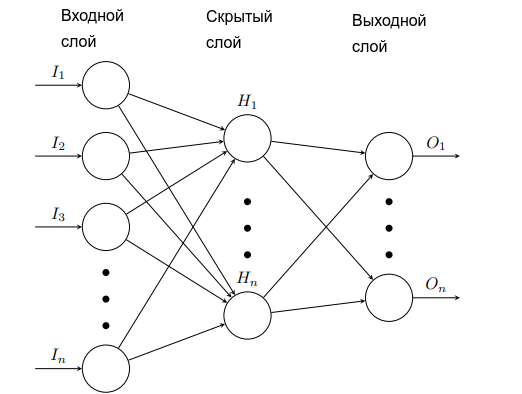
\includegraphics[width=.9\textwidth]{master_img/img1_edited.png}
	\caption{Трехслойная нейронная сеть с прямыми связями}
	\label{fig01}
\end{figure}
Каждая связь в сети имеет свой вес. Нейрон использует входные значения и веса чтобы посчитать выходное значение. Типичным методом композиции является  взвешенная сумма.

\begin{equation}
f(x)=K(\sum_iw_ix_i)
\end{equation}
Нелинейная функции активации К позволяет нейронной сети решать нетривиальный задачи, используя небольшое количество нейронов. Логистическая функция \ref{formula3} может использоваться в качестве функции активации.

Прогноз результата матча осуществляется на основе передачи в нейронную сеть неких свойств игрока и свойств матча. Если используется логичестическая функция активации, то выходное значение нейронной сети можно интерпретировать как вероятность выиграть матч. Есть большое количество различных алгоритмов обучения, которые оптимизируют набор весов нейронной сети в целях получении наилучшего выходного значения. Например, алгоритм обратного распространения использует градиентный спуск для уменьшения среднего квадрата ошибки между целевыми значениями и выходами сети.

Например, Сомбоонфокафан\cite{Book12} сконструировал трёхслойную сеть прямой связи, использую алгоритм обратного распространения ошибки. Протестировал на различных архитектурах сети и различных наборах свойств. Нейронная сеть, показавшая наилучший результат, имеет 27 входных нейронов. На вход подавались свойства, описывающие обоих игроков, а так же свойства матча. В результате была получена точность предсказания 75\% на исторических данных турниров "Большого шлема"\ в 2007-2008 годах.

Нейронная сеть можно установить наличие сложных взаимоотношений  между различными свойствами, подаваемыми на вход. Но она работает по принципу "черного ящика"\, т.е. механизм определения таких взаимоотношений не будет известен. К недостаткам нейронных сетей так же можно отнести то, что они склонны к переобучению, зачастую требует большого количества данных для обучения. Кроме того, разработка структуры сети зачастую является эмпирической и выбор гиперпараметров модели часто идёт методом проб и ошибок.
\subsubsection{Метод опорных векторов}
Основная идея метода опорных векторов заключается перевод исходных наборов свойств  в пространство более высокой размерности и поиск разделяющей гиперплоскости с максимальным зазором в этом пространстве. Две параллельных гиперплоскости строятся по обеим сторонам гиперплоскости, разделяющей классы. Разделяющей гиперплоскостью будет гиперплоскость, максимизирующая расстояние до двух параллельных гиперплоскостей. Алгоритм работает в предположении, что чем больше разница или расстояние между этими параллельными гиперплоскостями, тем меньше будет средняя ошибка классификатора.
На данный момент в открытом доступе нет работ по прогнозированию теннисных матчей при помощи метода опорных векторов\cite{Book13}. Метод опорных векторов имеет несколько преимуществ по сравнению с нейронными сетями. Во-первых, обучение не заканчивается на локальном минимуме, что зачастую бывает с нейронными сетями. Во-вторых, при наличии большого количество данных для обучения, метод опорных векторов обычно превосходит нейронные сети в прогнозировании \cite{Book13}. Тем не менее, время обучения модели метода опорных векторов намного выше, а создание и задание необходимых параметров модели является нетривиальной задачей.

\subsubsection{Проблемы машинного обучения}
Наличие большого количества данных для обучения не означает получение более точных результатов прогнозирования результатов теннисных матчей, т.к. большое количество данных означает, что теннисист играл много лет матчи. Со временем его навыки меняются и результаты последних матчей представляют набольший интерес. Так же в теннисе важную роль играет покрытие на которой играется матч, т.е. для модели необходимы данные о последних матча игрока именно на этом покрытии. Поэтому машинное обучение может страдать от недостатка данных, что может приводить к переобучению модели, с которым может быть сложно бороться. В частности нейронные сети сильно подвержены переобучению если количество слоёв/нейронов сравнительно велико относительно размера данных для обучения.

Чтобы бороться с проблемой переобучения, нужно использовать только важные свойства для обучения. Процесс отбора важный свойств набора данных называется "отбор признаков"\, для этого существует большое количество различных алгоритмов. Удаление незначащих свойств значительно уменьшает время обучения
\subsubsection{Оптимизация гиперпараметров}
Модель имеет параметры как получаемые в процессе обучения путём их оптимизации(например, веса в нейронных сетях), 
так и статически задаваемые параметры такие как количество скрытых слоёв, количество нейронов в каждом слое. Статически настраиваемые параметры называют гиперпараметрами. Процесс получения оптимальных гиперпараметров может быть как эмпирическим, так и алгоритмическим. Пример алгоритмического поиска гиперпараметров - поиск по сетке. Он происходит на заранее определённом пространстве гиперпараметров. Для построения модели прогнозирования с высокой точностью, необходимо тщательно подобрать необходимые гиперпараметры.

\subsubsection{Выбор оптимальных свойств}
Каждый набор данных может содержать большое количество различных свойств. Каждое свойство вносит определенный вклад в итоговый результат. Выбор оптимального количества наиболее значимых свойств - приём очень часто применяемый в машинном обучение. От количества свойств зависит производительность получаемой модели. Свойства, не влияющие на итоговый результат, или влияющие незначительно, негативно влияют на производительность модели, при включении их в оную. Так же нерелевантные свойства могут ухушить точность модели, заставить её обучаться на нерелевантных данных\cite{Book14}.

Преимущества выбора оптимального набора свойства
\begin{itemize}
	\item Уменьшает вероятность переобучения. Использование меньшего количества избыточных данных уменьшает вероятность принятия решения на основе "шума"\ .
	\item Повышение точности.
	\item Сокращает время обучения- меньшее количество данных снижают сложность модели.
\end{itemize}
Выбор свойств может производится как в ручном, так и автоматическом режиме.

Существуют 3 основных класса алгоритмов выбора свойств.
\begin{itemize}
\item Фильтр. Рассчитывается определенная метрика и свойства "фильтруются"\ на основании этой метрики
\item Обертка. "Оберточные"\ методы рассматривают выбор оптимального набора свойств
\end{itemize}

\textbf{Корреляция Пирсона} - фильтр-метод, который использует в качестве метрики следующую формулу:
\begin{equation}
\label{pearson}
r=\frac{\sum(x - \overline{x})(y - \overline{y})}{\sqrt{\sum(x - \overline{x})^2\sum(y - \overline{y})^2}}
\end{equation}

\textbf{Хи-квадрат метод} - фильтр-метод, который использует в качестве метрики следующую формулу:
\begin{equation}
\label{chi2}
\chi^2=\sum_{i=1}^n\frac{(O_i - E_i)^2}{E_i}
\end{equation}
Где $O_i$ - фактическое количество наблюдений класса i, а $E_i$ - ожидаемое количество наблюдений класса i, при условии отсутствия зависимости между свойством и ожидаемым значением.
Рассмотрим пример подсчёта метрики Хи-квадрат.
Предположим, у нас есть следующие данные
\begin{table}[!h]
	
	\caption{\label{tab:table1}Фактическое количество наблюдений результатов игроков}
	
	\begin{center}
\begin{tabular}{|l|l|l|l|}

\hline

  & Кол-во побед & Кол-во поражений & Всего \\
\hline
Игрок1  & 20 & 5 & 25 \\
\hline
Игрок2  & 40 & 35 & 75 \\
\hline
Всего  & 60 & 40 & 100 \\
\hline

\end{tabular}
		
\end{center}

\end{table}

Для того чтобы рассчитать значения $\chi^2$, рассчитаем "ожидаемое"\ значение в каждой ячейки, если бы свойства были действительно независимы. Для этого нужно просуммировать значения каждой строки и поделить на общее количество записей.
Получим следующую таблицу;
\begin{table}[!h]
	
	\caption{\label{tab:table2}Ожидаемое количество наблюдений результатов игроков}
	
	\begin{center}
\begin{tabular}{|l|l|l|l|}

\hline

  & Кол-во побед & Кол-во поражений & Всего \\
\hline
Игрок1  & 15 & 10 & 25 \\
\hline
Игрок2  & 45 & 25 & 75 \\
\hline
Всего  & 60 & 40 & 100 \\
\hline

\end{tabular}
		
\end{center}

\end{table}

\textbf{Лассо-метод(сокращение от англ. least absolute shrinkage and selection operator)} - встроенный метод. На основе линейной регрессии происходит пошаговый выбор оптимальных параметров модели.  Идея метода заключается в том, что накладывается ограничение на сумму абсолютных значений свойств модели, сумма должна быть меньше некоторого фиксированного значения. Для этого того, чтобы этого добиться, применяется методы сжатия(регуляризации), в процессе которого коэффициенты регрессионных переменных уменьшаются. Свойства, получившие в результате регуляризации нулевой коэффициент, отбрасываются.

\textbf{Методы на основе деревьев} относятся к классу встроенных методов. Например, для определения оптимального наборы свойств может использоваться алгоритму случайного леса. Принцип работы встроенных методов нетривиален и выходит за рамки данной работы, подробнее с их принципами работы можно ознакомится в \cite{Book15}
\subsection{Предварительная обработка данных}

Перед тем как начать с работать с данными, их нужно предварительно обработать.Данные могут хранится в числовом, текстовом виде, в формате изображений, аудио/видео файлов и других многочисленных форматах. Алгоритмы прогнозирования работают исключительно с числовыми данными. Поэтому данные в других форматах нужно перевести в числовой формат. В данной работе будет рассмотрен перевод текстовых данных в числовой вид. Перед переводом данных, их нужно предварительно очистить.



\begin{figure}[!h]
	\centering
	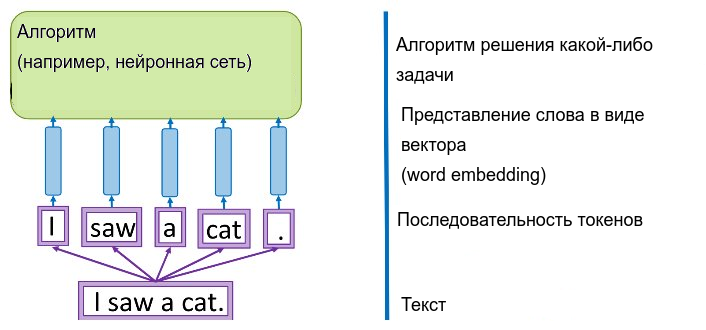
\includegraphics[width=.5\textwidth]{master_img/learning-word-representations_edited.png}
	\caption{Схема перевода текста в слова}
	\label{fig01_master}
\end{figure}

\subsubsection{One-Hot Encoding}
\begin{figure}[!h]
	\centering
	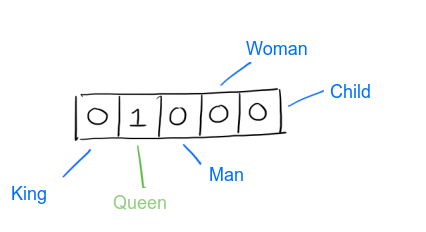
\includegraphics[width=.5\textwidth]{master_img/word2vec-one-hot_edited.png}
	\caption{Представление предложение "The queen entered the room"\ в виде вектора в формате one-hot encoding}
	\label{fig02_master}
\end{figure}
One hot encoding - это процесс в помощью которого некоторые категориальные  переменные(в нашем случае - слова), преобразуются в форму, понятную алгоритмам машинного обучения. Берется достаточно большой набор заранее известных слов(обычно речь идёт о десятках тысячах слов). На основании этого набора создаётся вектор чисел, где каждому слову соответствует  определенная позиция в этом векторе с изначальным  значением 0. Текст проверяется на наличие таких слов. Если слово присутствует  в тексте, то соответствующая  позиция устанавливает в 1, иначе в 0. На выходе получается разряженная матрица в виде вектора. Так же некоторые модификации этого метода используют размерности матрицы отличные от 1 по высоте.
К недостаткам данного метода можно отнести:
\begin{itemize}
	\item Большое количество затрачиваемой памяти. Текст из 40 слов и 4000 будут заниматься одинаковое количество место. Решается оптимизацией хранения разреженных матриц
	\item Потерю смысла слов. Одно и тоже слово может иметь несколько значений в зависимости от контекста
	\item Потерю порядка слов.
	\item Потеря количества определенных слов в тексте. Слово, употребленное в тексте один раз, имеет такой же вес, как и многократно употреблённое слово.
\end{itemize}
Так же к недостаткам стоит отнести трудоёмкость предварительной подготовки текста.
Для этого метода необходимо привести слова в один падеж, одно число.Например, "кота"\ - > "кот"\, "коты"\ -> "кошка"\ . Так же слова-синонимы заменяются на один конкретный вариант. Например, "автомобиль"->"машина". Это может быть нетривиально, особенно когда синонимы состоят из нескольких слов.

Основным преимуществом данного метода считается, что полученных данных достаточно для решения многих задач ествественной обработки языка\cite{Book26}, в частности классификации. Для многих задач анализа естественного языка вышеописанные недостатки несущественны. Так же такой формат данных удобен для работы с нейронными сетями и другими алгоритмами машинного обучения.

Развитием алгоритма one-hot encoding является так называемый "мешок слов"\ . Для его получения OHE-вектора каждого слова в тексте складываются. .е. на выходе получим просто подсчет количества различных слов в тексте в одном векторе. Такой подход называется "мешок слов"\ (bag of words, BoW), потому что мы теряем всю информацию о взаимном расположении слов внутри текста.
\begin{figure}[!h]
	\centering
	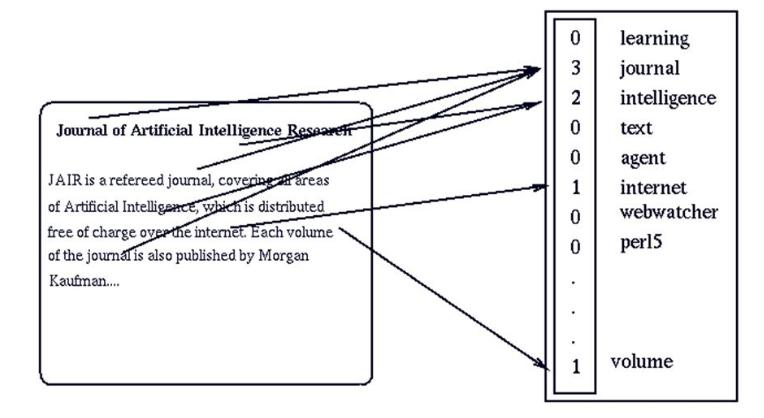
\includegraphics[width=.5\textwidth]{master_img/wordbag.jpg}
	\caption{Мешок слов}
	\label{fig03_master}
\end{figure}
\subsubsection{Dense Embedding Vectors}

Вышеописанные подходы были (и остаются) хороши для областей, где количество текстов мало и словарь ограничен, хотя, конечно, они имеют свои недостатки Но в современном мире количество слов огромно, слова постоянно появляются и исчезают С этим надо было что-то делать, а ранее известные модели не могли справиться с таким объемом текстов. Предположим, что в английском языке сейчас примерно около миллиона слов. Матрица совместных встречаемостей(такие матрицы используются для сравнения текстов) пар слов будет  иметь размер $10^6 x 10^6$. Такие матрицы занимают очень много памяти, с ними неудобно работать. Изобретено множество способов, упрощающих или распараллеливающих обработку таких матриц, всё-таки до сих пор с ними крайне тяжело работать\cite{Book27}.

Подход, решаюший данную проблему,  называется Dense Embedding Vectors
Этот подход основан на гипотезе, которую в науке принято называть гипотезой локальности — Эслова, которые встречаются в одинаковых окружениях, имеют близкие значенияЭ. Близость в данном случае понимается очень широко, как то, что рядом могут стоять только сочетающиеся слова. Например, для нас привычно словосочетание "заводной будильник". А сказать “заводной арбуз”  нельзя — эти слова не сочетаются.
Представим, что мы сожмём количество измерений вектора, используемого для представления миллиона уникальных слов с миллиона  до 50-100. При таком подходе каждое слово не будет иметь своего измерения, а будет отображаться на некий вектор.
Нейронная сеть вычисляет вероятность того, что определённое слово может встретиться в данном контексте.
\begin{figure}[!h]
	\centering
	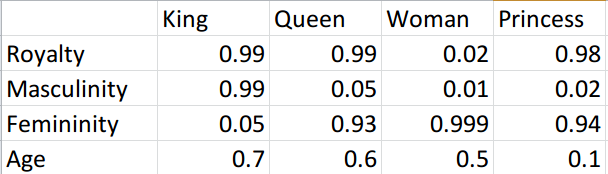
\includegraphics[width=.5\textwidth]{master_img/dense_emb_example_edited.png}
	\caption{Контекстные вероятности}
	\label{fig06_master}
\end{figure}

В 2013 году был предложен новый подход в Dense Embedding Vectors, названный word2vec.
Модель, предложенная Миколовым\cite{Book28}, проста. Она основывается на  предсказании вероятности слова по его окружению (контексту). То есть ожидается получение таких векторов слов, чтобы вероятность, присваиваемая моделью слову была близка к вероятности встретить это слово в этом окружении в реальном тексте.
Приведем формулу "мягкого максимума"\ (дифференцируемого). Максимум должен быть дифференцируем, чтобы модель могла обучаться при помощи алгоритма обратного распространения ошибки.
\begin{equation}
P(w_o|w_c) = \frac{e^{s(w_0, w_c)}}{\sum_{w_i \in V}e^{s(w_0, w_c)}}
\end{equation}
Где $w_0$ - вектор целевого слова, $w_c$  - некоторый вектор контекста вычисленный(например, путем усреднения) из векторов окружающих данное  слов, $s(w_1, w_2)$  - некая функция, получающая на вход 2 вектора и отображающая их в одно число. Например, это может быть функция косинусного расстояния.

Модель обучается следующим образом: берется последовательность 2k + 1 слов, где слово в центря является словом, которое должно быть предсказано. Окружащюие слова являеются контекстом длины K с каждой стороны от искомого слова. В процессе обучения каждому слову сопоставляется уникальный вектор, который меняется в процессе обучения.

Такой подход называется CBOW(англ. continuous bag of words). Является подвидом метода "мешка слов"\ т.к. порядок слов в контексте не учитывается. 

Так же существует развитие данного метода - skip-gram\cite{Book28}("словосочетание с пропуском"\ ). Оно основывается на том, что  из данного нам слова мы пытаемся "угадать контекст"\ . В остальном алгоритм не претерпевает измненений.

Натренированная модель word2vec может улавливать некоторые семантические и синтаксические свойства слов, несмотря на то что в модель явно не заложено никакой семантики.
\begin{figure}[!h]
	\centering
	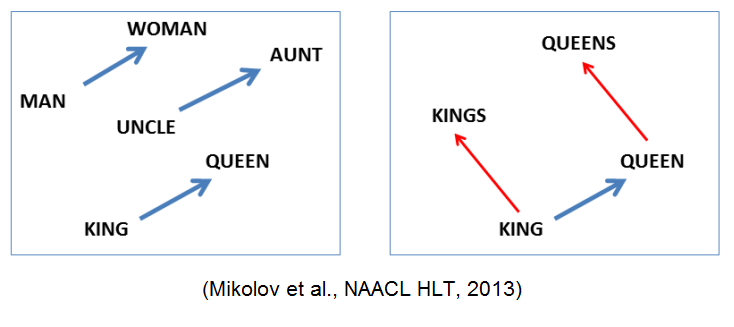
\includegraphics[width=.5\textwidth]{master_img/word2vec_example.png}
	\caption{word2vec пример семантической корреляции\cite{Book28}}
	\label{fig04_master}
\end{figure}
Слово "мужчина"(англ. man) относится к слову "женщина"(англ. woman) так же, как слово "дядя"(англ. uncle) к слову "тётя"(англ. aunt). Для человека это естественно и понятно, но в других моделях добиться такого же соотношения векторов можно только с помощью специальных ухищрений.
\subsubsection{Улучшения word2vec}
Модель CBOW c функцией оптимизации(минимизацией) в виде  дивергенции Кульбака-Лейблера называют моделью CBOW с negative sampling\cite{Book29}.
\begin{equation}
KL(p||q) = \int p(x)log\frac{p(x)}{q(x)}dx
\end{equation}
Где $p(x)$  — распределение вероятностей слов, а $q(x)$ - распределение словвзятое из модели(которая была получена на основе текста). Эта формула имеет описывает насколько одно распределение не похоже на другое(англ. divergence  - расхождение). Из-за того, что распределение получается на основе подсчёта слов, оно является дискретным. Поэтому  можно заменить интеграл на сумму:
\begin{equation}
KL(p||q) = \sum_{x \in V} p(x)log\frac{p(x)}{q(x)}dx
\end{equation}
К сожалению, эта формула имеет недостаток - большую вычислительную сложность. Прежде всего, из-за того, что $q(x)$ рассчитывается как softmax на основании всего словаря текста.
Именно поэтому Томасом Милковым\cite{Book29} была предложена оптимизация вышеприведенной формула, названная Negative Sampling. Как уже отмечалось ранее, очевидно, что многие слова вместе не встречаются. Поэтому большая часть вычислений в softmax являются избыточными. Это позволяет ввести следующую оптимизацию: максимизируется вероятность встречи слова для нужного слова в типичном для него контексте(в том котором он чаще всего встречается в заданном тексте). А вероятность встречи слова в нетипичном для него контексте, соотвественно, минимизируется.
\begin{equation}
NegS(w_0) = \sum{_{i=1, x_i \sim D}^{i=k} -log(1 + e^{s(x_i, w_0)})}  + 
\sum{_{j=1, x_j \sim D}^{i=k} -log(1 + e^{s(x_j, w_0)})}
\end{equation}
Где $s(x,w)$ - аналогичен оригинальной формуле,  D - hаспределение совместной встречаемости слова w и остальных слов текста. Формлуа состоит из двух частей - $+s(x,w)$ и негативной $-s(x,w)$. Позитивная часть отвечает за типичные контексты, а негативная за атипичные контексты(т.е. редкие словосочентания).
Они порождатся из распределения , $D`$ которое берется как равномерное по всем словам словаря корпуса. Было показано, что такая функция приводит при своей оптимизации к результату, аналогичному стандартному softmax\cite{Book29}.


Так же возможен вариант  оптимизации подсчёта модели word2vec через более эффективный подсчёт softmax. Например, используя дерево Хаффмана\cite{Book30}

Идея оптимизации заключается в том, что на основе словаря текста строится дерево Хаффмана, в каждом листе дерева слово, всего V слов. Пусть путь до слова w2 - L(w), а j-тая вершина по пути к w2 - n(w,j).
\begin{figure}[!h]
	\centering
	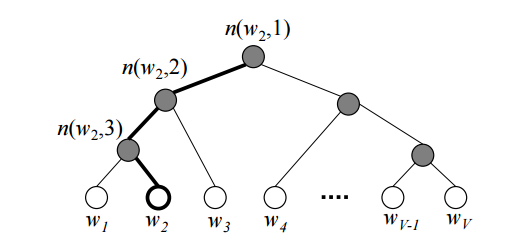
\includegraphics[width=.5\textwidth]{master_img/haffman.png}
	\caption{Дерево Хаффмана}
	\label{fig04_master}
\end{figure}
С помощью иерархического softmax вектора $u_{n(w,j)}$ можно рассчитать для V - 1 внутренних вершин.
Вероятность того, что w окажется выходным словом можно рассчитать по формуле:
\begin{equation}
p(w = w0) = \prod_{j=1}^{L(w) - 1} = \sigma([n(w,j + 1) = lch(n(w,j))]v^T_{n(w,j)}u)
\end{equation}
Где $\sigma(x)$ - функция softmax, lch(n) - левый сын вершины n, $u=v_{wI}=\frac{1}{h}\sum^h_{k=1}v_{wI,k}$ т.е. усредненный вектор контекста при использовании CBOW.

Стандартный алгоритм softmax имеет ассиптотическую сложноность O(V). Улучшенный алгоритм softmax позволяет вычислисть вероятность слова при помощи последовательных вычислений за O(log(V)).

\subsubsection{Недостатки Dense Embedding Vectors}
Методы Dense Embedding Vectors изначально были придуманы для английского языков, то там не так остро стоит проблема словоизменения для славянских языков.  В вышеописанных методах предполагается, что разные формы одного слова считаются одним словом. Только тогда нейронная сеть сможет установить корректно семантические и синтаксические связи. Чтобы избежать проблем при формирования связей, используют стеммирование(обрезание окончания слова, оставление только основы) и/или лемматизация(замену слова его начальной формой) 
 на этапе предварительной подготовки текста.
 
\subsection{Нормализация данных} 
После получения предварительно обработанного датасета для обучения модели, данные необходимо нормализовать. Нормализация данных предназначена для устранения зависимости от выбора единицы измерения и заключается в преобразовании диапазонов значений всех атрибутов к стандартным интервалам([0,1] или [-1,1])\cite{Book25}. Нормализация данных направлена на придание всем атрибутам одинакового "веса".

Рассмотрим основные методы нормализации данных.
\begin{enumerate}
	\item Min-max нормализация заключается в применении к диапазону значений атрибута х линейного преобразования, которое отображает [min(х),max(х)] в [A,B].
	\begin{equation}
	\label{mixmaxNorm}
	x^\prime_i=\uptau(x_i)=\frac{x_i - min(x)}{max(x) - min(x)}*(B-A) + A
	\end{equation}
	\begin{equation}
	x \in[min(x), max(x)] \Rightarrow \uptau(х) \Rightarrow [A,B]
	\end{equation}
	Min-max нормализация сохраняет все зависимости и порядок оригинальных значений атрибута. Недостатком этгого метода является то, что выбросы могут сжать основную массу значений к очень маленькому интервалу
	\item Z-нормализация  основывается на приведении распределения исходного атрибута х  к центрированному распределению со стандартным отклоненим, равным 1 \cite{Book25} .
	\begin{equation}
	\label{ZNormalization}
	x^\prime_i=\uptau(x_i) =\frac{x_i - \overline{x}}{\sigma_x}
	\end{equation}
	\begin{equation}
	M[x^\prime]=1	 
	\end{equation}
	\begin{equation}
	D[\overline{x}^\prime]=0	 
	\end{equation}
	Метод полезен когда в данных содержатся выбросы.
	\item Масштабирование заключается в изменении длины вектора значений атрибута путем умножения на константу \cite{Book20} .
	\begin{equation}
	x^\prime_i=\uptau(x_i)=\lambda*x_i
	\end{equation}
	Длина вектора х уменьшается при $|\lambda|<1$ и увеличивается при $|\lambda|>1$ 
\end{enumerate}
\subsection{Выводы}

\begin{table}[!h]
	
	\caption{\label{tab:table3}Точность прогнозов различных методов}
	
	\begin{center}
		\begin{tabular}{|l|l|l|}
			
			\hline
			
		 Название метода	& Точность прогноза & Возможн. модификации \\
			\hline
			Метод подсчёта очков  & 60-65\% & Низкая \\
			\hline
			Методы попарного сравнения  & 63-67\% & Средняя  \\
			\hline
			Методы машинного обучения  & 69\%+ & Высокая  \\
			\hline
			
		\end{tabular}
		
	\end{center}
	
\end{table}
Существует большое количество алгоритмом прогнозирования результатов спортивных соревнований и теннисных матчей в частности. Однако, современные разработки в основном ведутся в области машинного обучения, в частности  популярны нейронные сети. Методы на основе нейронных сетей гибки и позвляют легко разрабатывать собственные модификации уже известных методов.

Алгоритмы могут использовать в качестве входных данных как числовые данные, так и текстовые данные, переведенных в вид чисел.
 При этом для перевода текстовых данных  в численный вид оптимально использовать современные методы word embedding такие как word2vec.
 Область знаний прогнозирования спортивных соревнований и в частности прогнозирования результатов теннисных
 матчей активно развивается как часть современной науки, остается ещё много простора для исследования алгоритмов, модификации и со­здания новых.
 
Анализ текста будет проводится на основе англоязычных текстов в связи с тем, что современные алгоритмы заточены на работу с английским языком, а также большинство данных о теннисе представлены на английском языке.